
\begin{figure}[h!]
	\centering
	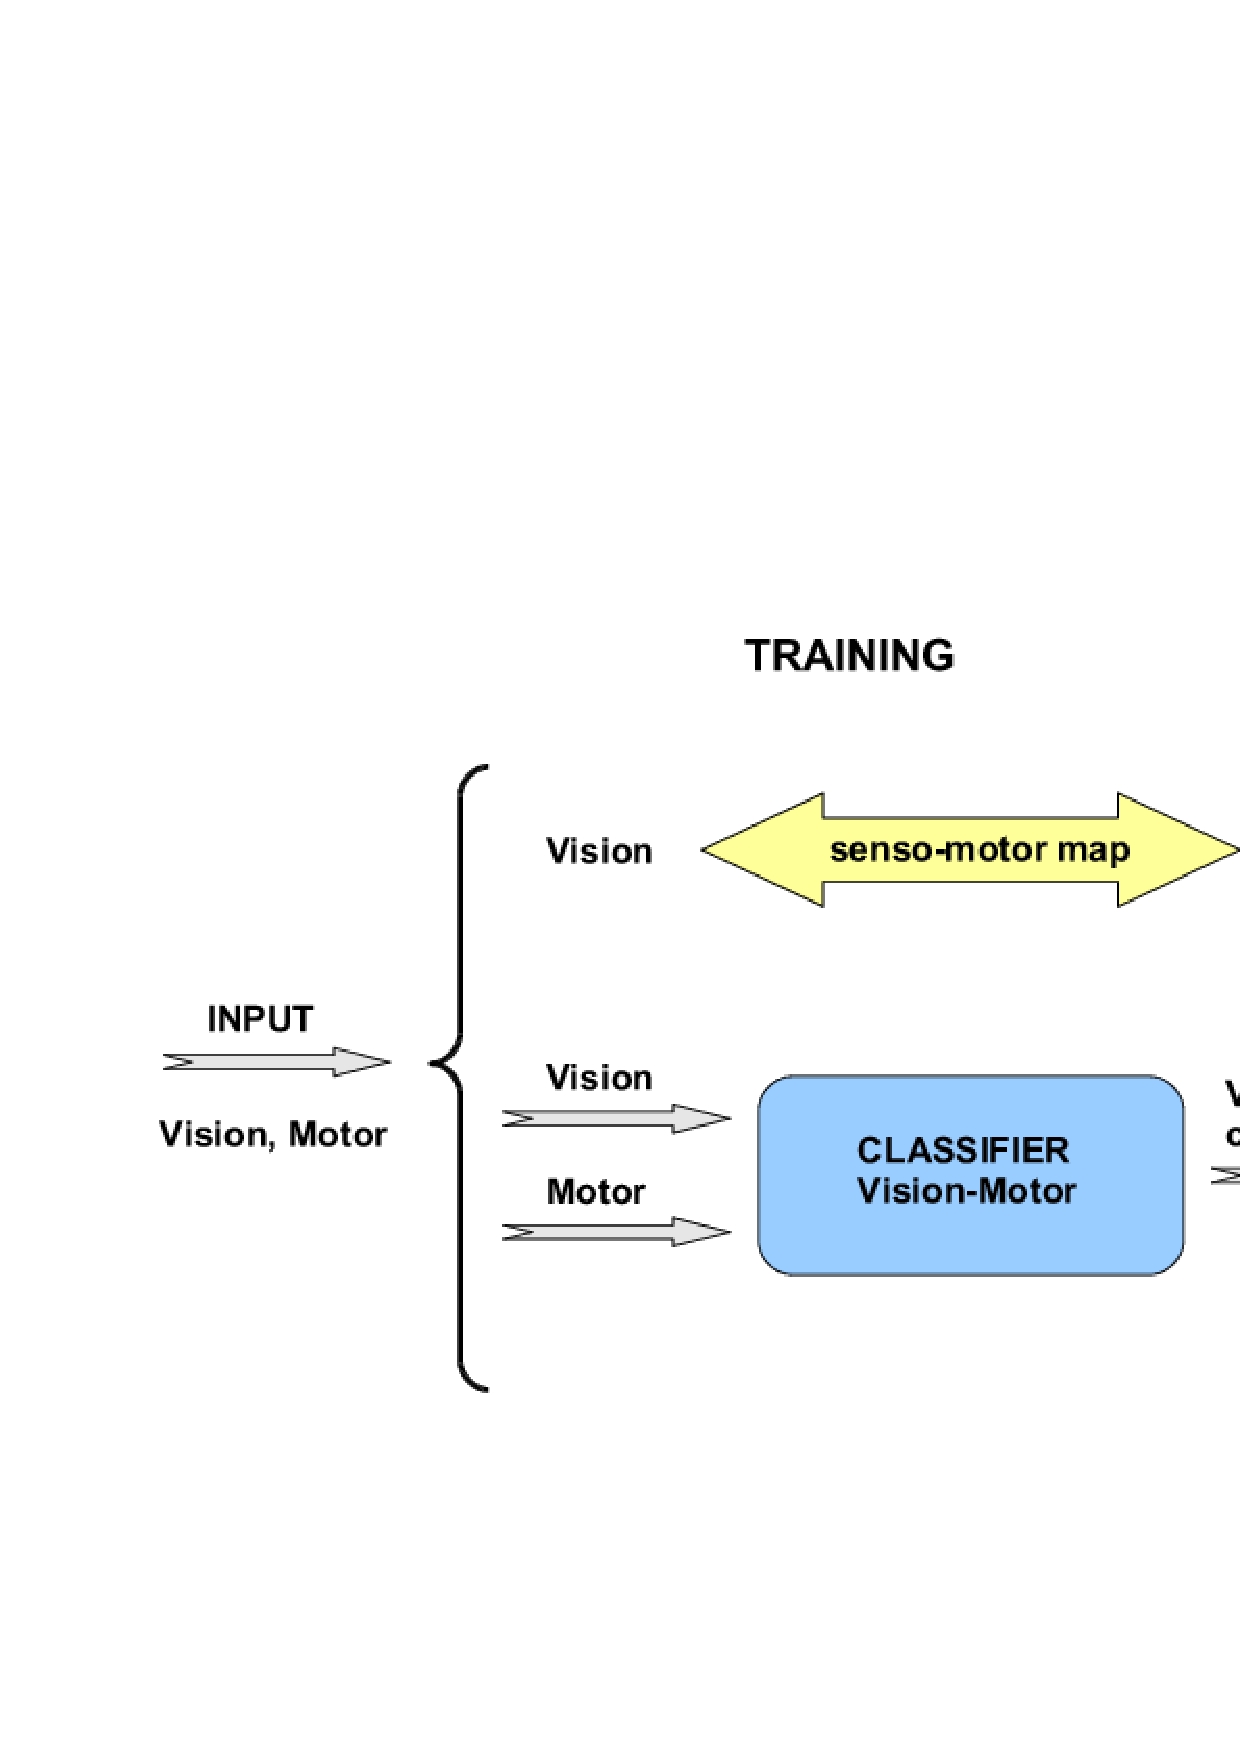
\includegraphics[width=0.7\textwidth]{images/train_fig}
	\caption{blabla}
	\label{fig:training-scheme}
\end{figure}

\begin{figure}[h!]
        \centering
        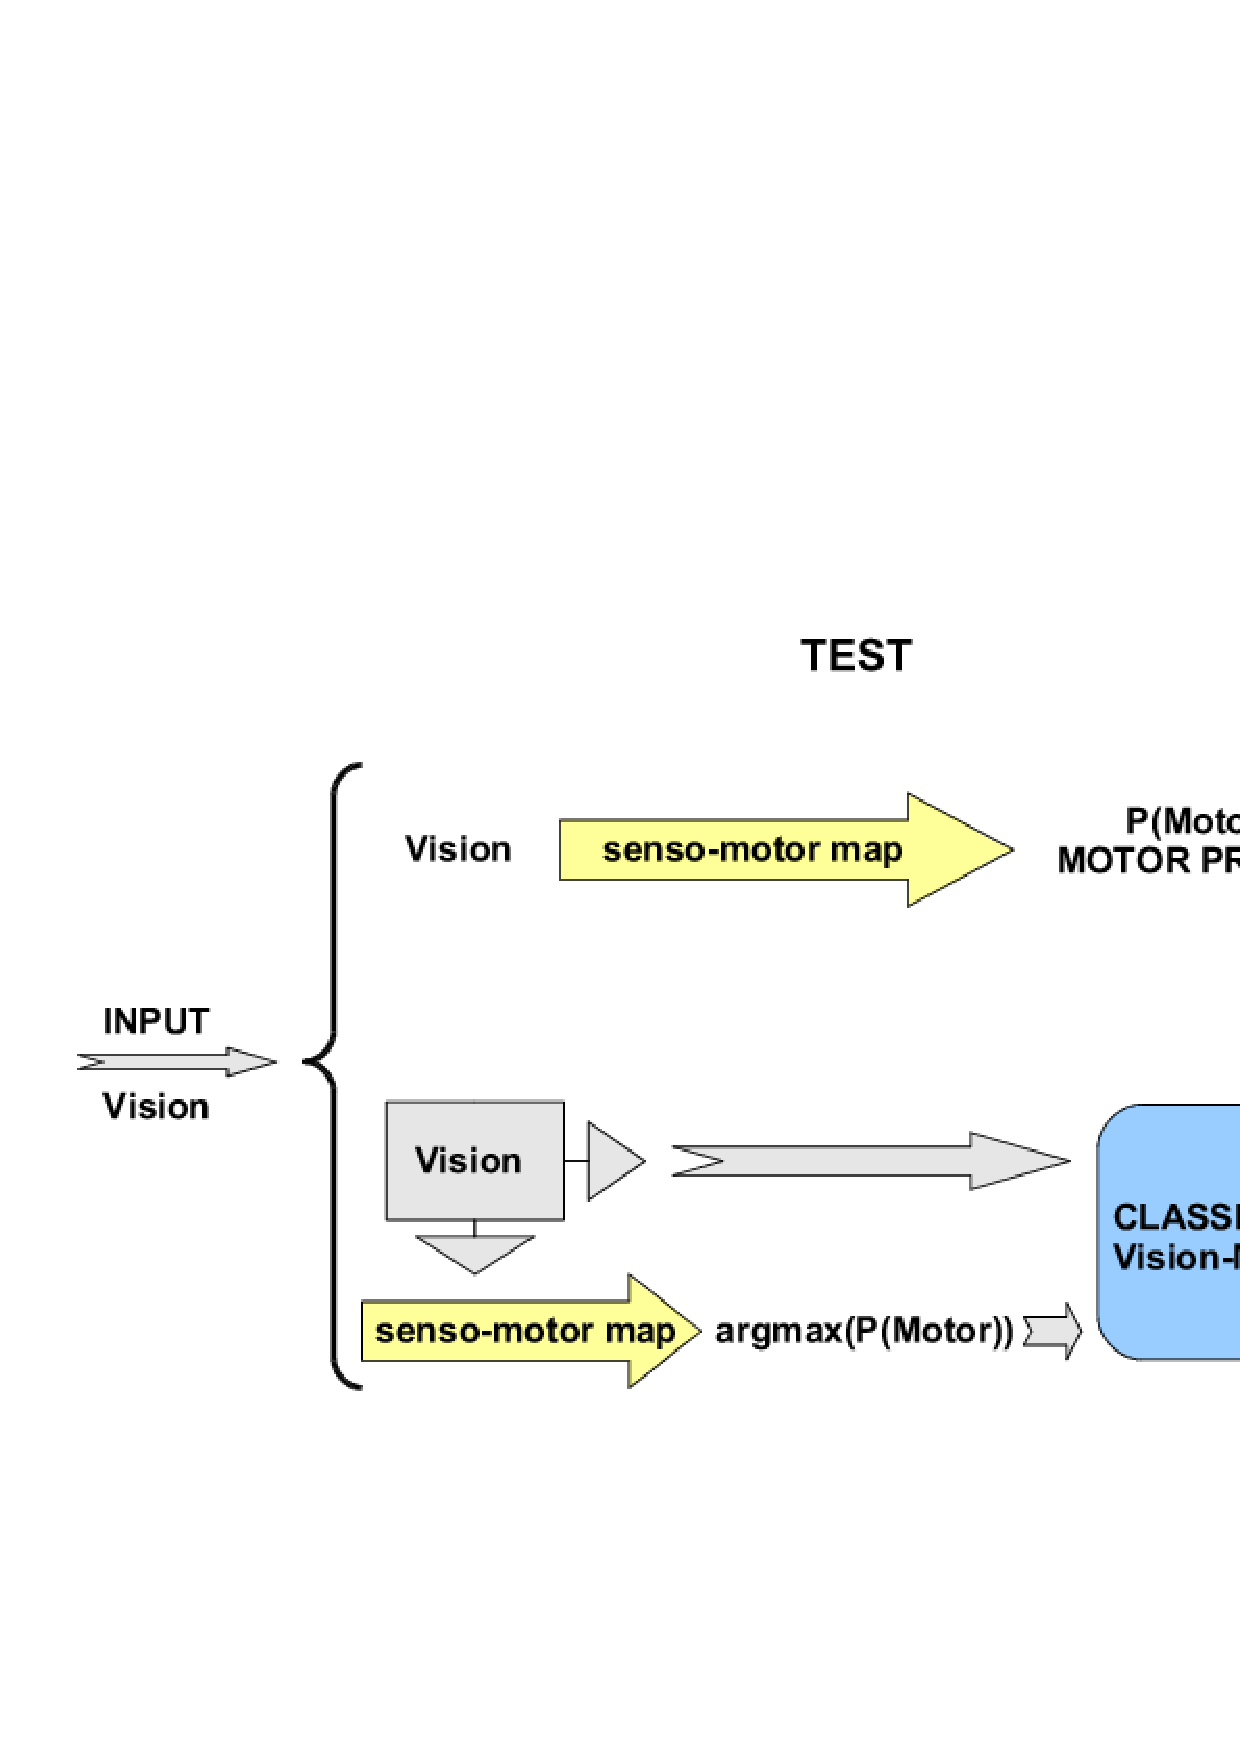
\includegraphics[width=0.7\textwidth]{images/test_fig}
        \caption{blabla}
        \label{fig:test-scheme}
\end{figure}


%\vskip -0.5cm

The training phase is schematically illustrated in Figure \ref{fig:training-scheme}. During training, the system receives as input labeled visual and motor
perceptual representation. These correspond to the seen object (Visual Perceptual Representation, VPR) and to the grasp posture of the hand
manipulating the object (Motor Perceptual Representation, MPR). On these data, the system builds in parallel two functions: a senso-motor map
between VPR and MPR (Figure \ref{fig:test-scheme}, top) and a classification function receiving as input both modalities, trained
to recognize the perceived object (Figure \ref{fig:training-scheme}, bottom). Technical details on how we compute the sensor motor map and the
multi-modal classifier are reported in section .. and ...

Figure \ref{fig:test-scheme} shows the test phase with its two possible outcomes. When receiving as input a VPR of a known object, the system can
opt for two different types of action:
\begin{itemize}
\item {\em Activation of the sensor-motor map}. This produces as an output an estimate of the most probable motor grasps associated 
to that object, with the corresponding 
MPRs for the grasp postures. We call this estimates {\em motor priming}, as they would correspond in an embodied agent to the pre-activation of the possible 
grasps. A detailed description of how we obtain the motor priming is given in section .....

\item {Object classification}. Note that, having learned the object on two modalities, the classifier needs as input a VPR and its corresponding MPR. We derive the
{\em not perceived} MPR using the senso-motor map (Figure \ref{fig:test-scheme}, bottom). The obtained motor priming is then given as input to the classifier with the VPR. We stress again that the clasifier recognizes the object on the basis of its visual appearance and of how it can be grasped. Experiments
reported in section ... shows clearly that this leads to a significant increase in performance compared to using only visual information.

\end{itemize}

